\documentclass[portrait]{poster}

\usepackage{minted}
\begin{document}

\printheader

\begin{center}
    %% TITLE
    \textbf{\bf\veryHuge\color{NavyBlue}Practical usage of Zero-knowledge in different use-cases in blockchains\\[1.5cm]}

    %% AUTHORS
    \huge     Lukáš Častven \\[0.2cm]
    \Large    \texttt{xcastven@stuba.sk}
\end{center}

\vspace{2cm}

\Large

\begin{multicols}{2} % begin two columns

\section*{Introduction}

    Zero Knowledge Proofs (ZKPs) provide a unique way to prove information without
    actually revealing the information itself. This makes them ideal for
    enhancing anonymity and privacy in blockchain networks. This work
    explores the use of ZKPs to create stealth addresses on Ethereum blockchain.

    ZKPs replace elliptic curve cryptography in stealth address schemas.
    This provides another method for proving ownership of a stealth
    address while protecting the recipient's identity.

\section*{Contributions}

    \begin{enumerate}
        \item \textbf{Blockchain Privacy Advancement:} This work highlights the power
            of ZKPs in developing privacy-focused cryptocurrency solutions.
        \item \textbf{ZKPs for Stealth Addresses:} Successful demonstration of using
            ZKPs in designing stealth address schema.
        \item \textbf{Trustless Ownership Proof: } Proposed scheme enables trustless
            proof of stealth address ownership without compromising privacy.
    \end{enumerate}

\section{Solution Design}

    Public blockchains expose transaction details, compromising privacy.
    stealth addresses enable anyone to send private transactions,
    while hiding recipient identities.

    The core principle behind the solution is that both receiver
    and sender generate a random value. These two values can then
    be used to prove to a stealth address that whoever owns these
    values is the owner of the stealth address, and can control it.

    Bob, as a receiver, publishes the hash of his random value to a public
    registry. With this hash he also publishes his public key, which corresponds
    to his private key. This tuple is Bob's meta stealth address, visualized in Figure
    \ref{fig:bobs-meta-address}.

    \begin{center}\vspace{1cm}
        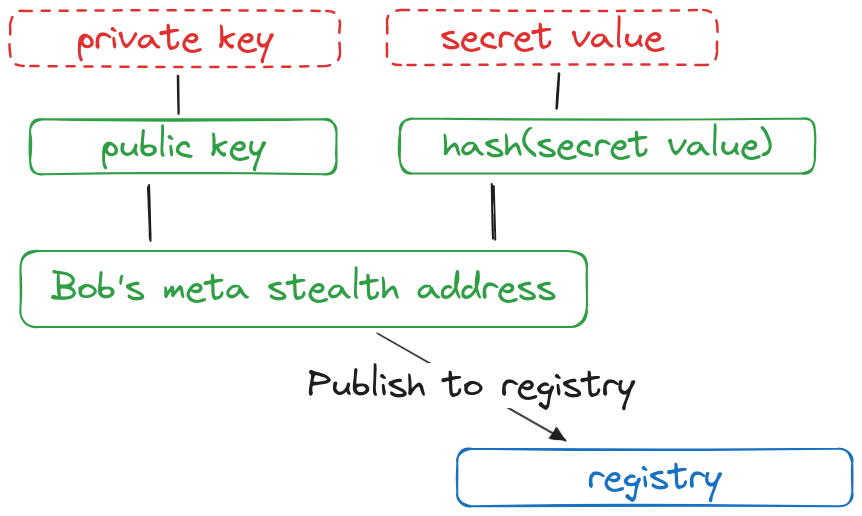
\includegraphics[width=0.5\linewidth]{../iitsrc/assets/images/meta-stealth-address.png}
        \captionof{figure}{Bob's Meta Stealth Address}
        \label{fig:bobs-meta-address}
    \end{center}\vspace{1cm}

    When Alice wants to send funds to Bob, she finds his meta stealth address
    in the public registry, generates her own random value and hashes it together
    with Bob's hash to create a code. Then she deploys a new stealth wallet
    contract with this code in it, and amount of funds that she wanted to send
    to Bob. After that, she encrypts her random value with Bob's public key,
    this encrypted value is called ephemeral key. Alice publishes it to a
    public registry. This whole process is depicted in Figure \ref{fig:sending-funds}. 

    \begin{center}\vspace{1cm}
        \centering
        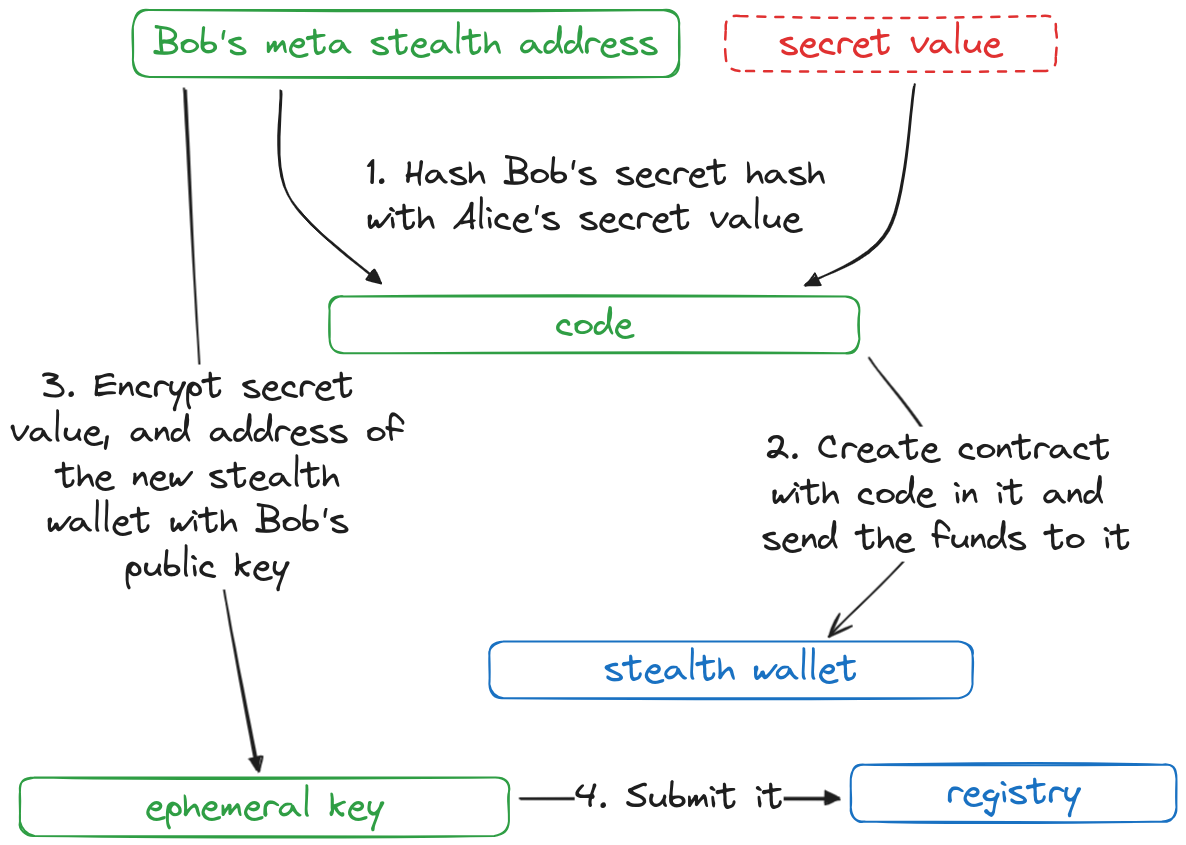
\includegraphics[width=0.7\linewidth]{../iitsrc/assets/images/sending-funds.png}
        \captionof{figure}{Alice sends funds}
        \label{fig:sending-funds}
    \end{center}\vspace{1cm}

    Bob then scans the registry, tries to decrypt ephemeral keys. When the
    decryption is successful, Bob can save the decrypted Alice's secret value
    and the address of the corresponding stealth wallet.

    \begin{center}\vspace{1cm}
        \centering
        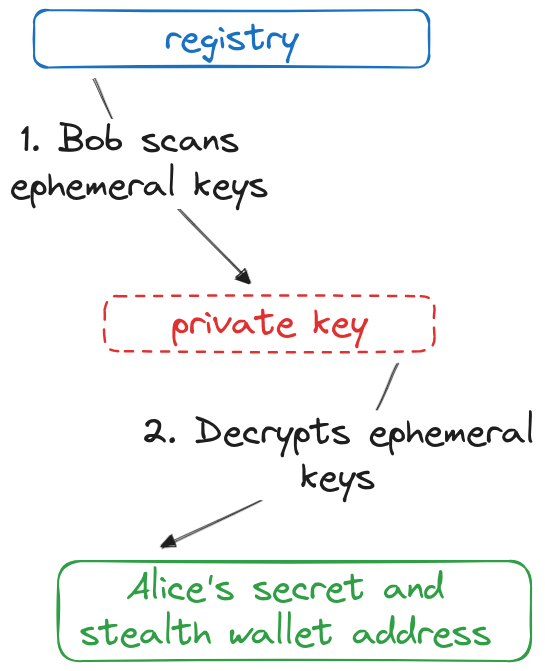
\includegraphics[width=0.5\linewidth]{../iitsrc/assets/images/scanning-ephemeral-keys.png}
        \captionof{figure}{Bob scans ephemeral keys}
        \label{fig:scanning-ephemeral-keys}
    \end{center}\vspace{1cm}


    To use the funds, Bob must generate a ZK proof and submit it to the stealth
    wallet. This proof proves that Bob knows Alice's random value
    and his own random value, such that
    \[ code = hash(hash(Bob's\:value),\:Alice's\:value) \]
    where $code$ is the one submitted by Alice into the stealth wallet contract.

    \begin{center}\vspace{1cm}
        \centering
        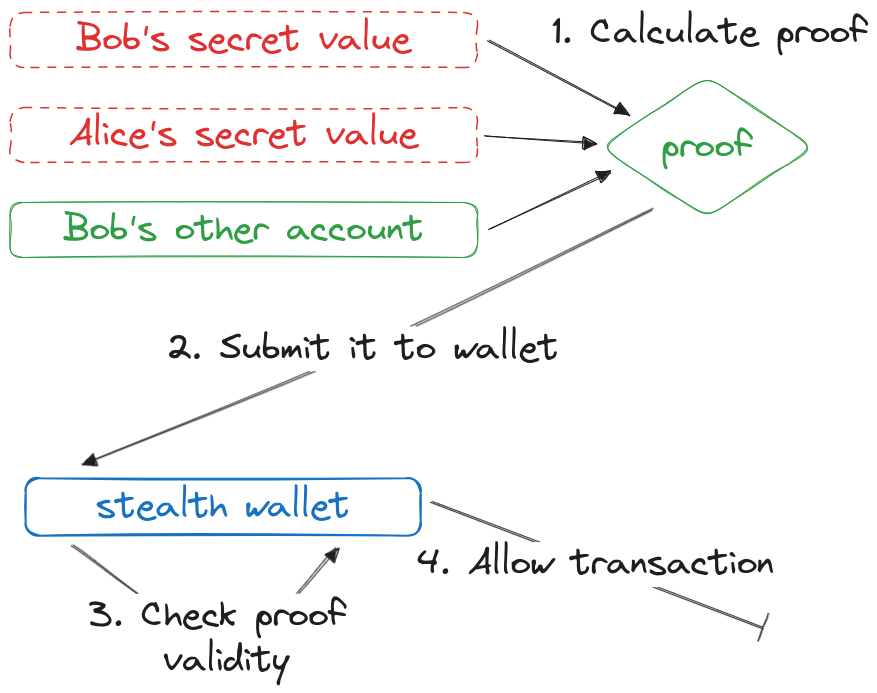
\includegraphics[width=0.5\linewidth]{../iitsrc/assets/images/interating-with-wallet.png}
        \captionof{figure}{Bob's interaction with wallet}
        \label{fig:wallet-interaction}
    \end{center}\vspace{1cm}

    \begin{minted}[fontsize=\small]{c}
pragma circom 2.0.0;

include "./circomlib/circuits/poseidon.circom";

template Ownership() {
    signal input owner_secret;
    signal input sender_secret;
    signal input code;
    signal input withdrawee_address;
    signal input msg_sender;

    log("input owner_secret:", owner_secret);
    log("input sender secret:", sender_secret);
    log("input code:", code);
    log("input withdrawee_address:", withdrawee_address);
    log("input msg_sender:", msg_sender);

    component owner_secret_poseidon = Poseidon(1);
    owner_secret_poseidon.inputs <== [owner_secret];
    log("calculated owner_secret hash:", owner_secret_poseidon.out);

    component code_poseidon = Poseidon(2);
    code_poseidon.inputs <== [owner_secret_poseidon.out, sender_secret];
    log("calculated code:", code_poseidon.out);

    code === code_poseidon.out;
    msg_sender === withdrawee_address;
}

component main {public [code, msg_sender]} = Ownership();
    \end{minted}

\section{Conclusions || Discussion}

O manual do \TeX~\cite{knuth1986} pode ser usado para aprendê-lo, e o livro do
Lamport~\cite{lamport1994} para aprender o \LaTeX, mas se quiser ir a fundo tem
que ver como o \TeX quero o os parágrafos em linhas~\cite{knuth1981}.

Two typesLorem ipsum dolor sit amet, consectetur adipiscing elit, sed
do eiusmod tempor incididunt ut labore et dolore magna aliqua. Uore eu
fugiat nulla pariatur. Excepteur sint occaecat cupidatat non proident,
sunt in culpa qui officia deserunt mollit anim id est laborum.



\begin{itemize}
\item Pellentesque eget orci eros. Fusce ultricies, tellus et
  pellentesque fringilla, ante massa luctus libero, quis tristique
  purus urna nec nibh. 
\item Vestibulum sem ante, hendrerit a gravida ac, blandit quis magna.
\end{itemize}

\bibliographystyle{plain}
\bibliography{refs}

\end{multicols}
\end{document}
